\chapter{Variabili Aleatorie}

Questo capitolo è dedicato a uno dei pilastri fondamentali della teoria della probabilità: le variabili aleatorie. Tale approfondimento ci permetterà di comprendere il motivo per cui si è reso necessario rivedere le funzioni e definire una notazione più adatta al contesto probabilistico.\\
\\
Abbiamo già introdotto che cosa è una misura e cosa sia uno spazio misurabile, ma quando possiamo dire che una \textit{funzione è misurabile}?
\begin{definizione}
    Siano $(E, \mathcal{E}), \;(F, \mathcal{F})$ due spazi misurabili; $f:E\to F$ si dice misurabile se $\forall B\in\mathcal{F}:\quad f^{-1}(B)\in \mathcal{E}$.\\
    \\
    Come notazione useremo: $f:E\to F$ misurabile, oppure $f:(E, \mathcal{E})\to (F, \mathcal{F})$
\end{definizione}
\noindent Come abbiamo già notato in precedenza, per qualsiasi funzione vale che:
\[\set{X^{-1}(B)\mid B\subseteq \mathcal{F}}\subseteq \mathcal{P}(\Omega)\]
Tuttavia \textit{se parliamo di funzioni misurabili} siamo in grado di creare una condizione più forte sull'insieme delle controimmagini\footnote{Si ricorda che $\mathcal{E}\subsetneq \mathcal{P}(\Omega)$}:
\[\set{X^{-1}(B)\mid B\subseteq \mathcal{F}}\subseteq \mathcal{E}\subsetneq \mathcal{P}(\Omega)\]

\begin{definizione}[\faWarning]
    Sia $(\Omega, \mathcal{A}, \mathbb{P})$ uno spazio di probabilità e $(F, \mathcal{F})$ uno spazio misurabile. Allora $X$ è una variabile aleatoria se:
    \[X:\Omega\to F \;\text{ è misurabile}\]
    Ossia che $\;\forall B\in \mathcal{F}: \quad X^{-1}(B) =: (X = B)\in \mathcal{A}$
\end{definizione}
\noindent Questa è una definizione generale, ma tipicamente per i nostri scopi avremo che:
\[F = \mathbb{R}, \mathbb{R}^n\quad \text{e}\quad \mathcal{F} = \mathcal{B}(\mathbb{R}), \mathcal{B}(\mathbb{R}^n)\]
Facciamo alcuni esempi per approfondire al questione:\\
\\
\(\bigstar\) Siano $\Omega = \set{1, ..., 6}^2 = \set{w\in (h, k): \;h, k\in\{1, ..., 6\}}, \;\mathcal{A} = \mathcal{P}(\Omega), \;F = \mathbb{R} \text{ e } \mathcal{F} = \mathcal{B}(\mathbb{R})$.\\
\\
È evidente che questa costruzione si rifà all'esperimento del lancio di 2 dadi. Possiamo quindi una funzione che ci restituisce la somma dei due risultati:
\[X(w) = h + k\]
Ci chiediamo, \textit{questa funzione è una variabile aleatoria?} Per esserlo, dobbiamo dimostrare $\;\forall B\in \mathcal{F}: \quad (X = B)\in \mathcal{A}$. \\
Siccome la $\sigma$--algebra di partenza è l'insieme delle parti, la condizione di misurabilità è sempre verificata, in quanto $(X\in B)\in \mathcal{P}(\Omega)$.\\
\\
Abbiamo appena capito che \textbf{tutte le volte che $\boldsymbol{\Omega}$ è discreto} (e quindi $\mathcal{A} = \mathcal{P}(\Omega)$), avremo che \textbf{la condizione di misurabilità è verificata automaticamente}, e quindi possiamo parlare di variabile aleatoria.\\
\\
Se avessimo invece preso $\tilde{\mathcal{A}} = \{\varnothing, \Omega\}$, la nostra funzione $X(w) = h+k$ non sarebbe più risultata misurabile. È facile da dimostrare, prendendo per esempio $B = \{2\}: \quad (X\in B) = (X = 2) = \{(1, 1)\}\notin\mathcal{A}$. $X$ non sarebbe quindi stata una variabile aleatoria.\\
\\
\(\quad\Rightarrow\) Tutto dipende dalle $\sigma$--algebre!!!\\
\\
\(\bigstar\) Prendiamo $\Omega = \mathbb{R}^+, \;F = \mathbb{R}, \; \mathcal{A}= \mathcal{B}(\mathbb{R}^+), \; \mathcal{F}= \mathcal{B}(\mathbb{R})$. Consideriamo
\[X:\mathbb{R}^+\to\mathbb{R}\quad\text{tale che}\quad X(w) = \lfloor w \rfloor+1\]
dove con $\lfloor x \rfloor$ si intende la parte intera di $x$.\\
Di nuovo ci chiediamo se questa possa essere una variabile aleatoria, ossia $\;\forall B\in \mathcal{F}: \quad (X = B)\overset{?}{\in} \mathcal{A}$?\\
Per aiutarci, andiamo a vedere come si comporta graficamente la funzione $X$:

\begin{figure}[H]
\centering
\begin{tikzpicture}[y=0.7cm, >=stealth]

% --- Assi ---
\draw[->, thick] (0,0) -- (5.2,0) node[right] {$\omega$};
\draw[->, thick] (0,0) -- (0,4.6) node[above] {$X$};

% --- Segmenti a gradini ---
\foreach \x/\y in {1/1, 2/2, 3/3, 4/4}{
    \draw[red, thick] (\x-1,\y) -- (\x,\y);
    \fill[red] (\x-1,\y) circle (1.3pt);
}

% --- Linea di continuazione del grafico ---
\draw[red, thick, dashed] (4,5) -- (5,5);
\fill[red] (4, 5) circle (1.3pt);


% --- Etichette numeriche sull'asse X ---
\foreach \x in {1,2,3,4}{
  \node[below=2pt] at (\x,0) {\small $\x$};
}

% --- Etichette numeriche sull'asse X ---
\foreach \y in {1,2,3,4}{
  \node[left=2pt] at (0,\y) {\small $\y$};
}

% --- Assi tratteggiati---
\foreach \x in {1,2,3,4}{
    \draw[dashed, gray!70] (\x,0) -- (\x,\x+1);
}


\end{tikzpicture}
\end{figure}

Grazie al grafico notiamo che $X(\Omega) = \mathbb{N^*}$, e di conseguenza possiamo scrivere che:
\[(X\in B) = \bigcup_{k\geq1; \;k\in B}(X=k)\]
Per capire meglio la scrittura, poniamo per esempio $B = (\frac{3}{2}, \frac{9}{2})$, allora ai avrà che:
\[(X\in B) = (X=2)\cup(X=3)\cup(X=4) = [1, 2)\cup [2, 3)\cup [3, 4)\]
In generale possiamo quindi scrivere che: 
\begin{align*}
    (X=k) &= \left(w:\;X(w) = \lfloor w\rfloor + 1 = k\right) = \left( w:\; \lfloor w\rfloor = k-1\right)\\
    &= [k, k-1)\quad \forall k \geq1
\end{align*}
Di conseguenza avremo che la condizione di misurabilità riuslta soddisfatta, difatti:
\[(X\in B) = \bigcup_{k\geq1; \;k\in B}(X=k) = \bigcup_{k\geq1; \;k\in B}[k, k-1)\in \mathcal{B}(\mathbb{R}^+) = \mathcal{A} \quad \forall B \in \mathcal{F} = \mathcal{B}(\mathbb{R})\]
\\
\noindent Da questo esempio capiamo che \textbf{se l'immagine di $\boldsymbol{X}$ è numerabile e lavoro sui Boreliani, allora $\boldsymbol{X}$ è una variabile aleatoria.}

\bigskip
\noindent
\begin{tikzpicture}
  \draw[dashed] (0,0) -- (\textwidth,0);
\end{tikzpicture}\\
\\
Ora che abbiamo introdotto e capito cosa è una variabile aleatoria, andiamo ad elencare tutte le sue principali proprietà.

\begin{teorema}[Proprietà delle Variabili Aleatorie\footnote{In generale delle funzioni misurabili}]
    Sia $(\Omega, \mathcal{A}, \mathbb{P})$ uno spazio di probabilità, e $(E, \mathcal{E}), \;(F, \mathcal{F})$ due spazi misurabili. Allora valgono le seguenti:
    \begin{enumerate}
    \label{th:propVA}
        \item $X:\Omega\to\mathbb{R}$: \\
        \[\text{V.A. reale} \quad\iff\quad(X\leq t) = (X\in (-\infty, t))\in \mathcal{A}\quad \forall t\in\mathbb{R}\]
        \item $X=\mathbb{I}_A:\Omega\to \mathbb{R}$:
        \[\text{V.A. reale} \quad\iff\quad A\in\mathcal{A}\]
        \item $\ve{X} = (X_1, ..., X_n):\Omega\to\mathbb{R}^n$:
        \[\text{Vettore A.}\quad \iff \quad X_k:\Omega\to \mathbb{R} \;\;\text{ è V.A. }\;\;\forall k = 1, ..., n\]
        \item Siano $X:\Omega\to E,\;\; h:E\to F$ misurabili:
        \(\quad \Rightarrow\quad Y = h\circ X:\Omega\to F\;\;\text{ è una V.A.}\)\\
        \\
        Ovvero che: \((Y \in C) = (h\circ X\in C) = (X\in h^{-1}(C))\), con \(C\in\mathcal{F}\). Siccome $h$ è misurabile: \( h^{-1}(C)\in\mathcal{E}\), e $X$ è misurabile: \(\Rightarrow(X\in h^{-1}(C))\in\mathcal{A}\)
        \item Sia $X_k:\Omega\to\mathbb{R}$ V.A. $\forall k=1, ..., n$. Sia $h:\mathbb{R}^n\to \mathbb{R}$:
        \[\overset{3.+4.}{\Rightarrow} h(X_1, ..., X_n) = h\circ \ve{X}:\Omega\to\mathbb{R}\quad \text{è una V.A.}\]
        \item Siano $X, Y:\Omega\to\mathbb{R}$ variabili aleatorie reali:
        \[\Rightarrow\quad X+Y,\; X-Y, \;XY,\; \frac{X}{Y}\mathbb{I}_{[Y\neq0]},\;X \vee Y,\;X \wedge Y \quad \text{Sono V.A.}\]
        \item Sia $X_n:\Omega\to \mathbb{R}$ una successione di variabili aleatorie:
        \[\Rightarrow\quad \sup_nX_n, \; \inf_nX_n, \;\lim_{n\to+\infty}X_n, \; \liminf_n X_n, \; \limsup_nX_n\quad \text{Sono V.A.}\]
        (Dove si ricorda che il ``$\liminf$'' e ``$\limsup$'' esistono sempre, mentre il ``$\lim$'' non è detto).
    \end{enumerate}
\end{teorema}
\begin{definizione}
    La funzione $\;h:(\mathbb{R}^n, \mathcal{B}(\mathbb{R}^n))\to (\mathbb{R}^k, \mathcal{B}(\mathbb{R}^k))$ si definisce \textit{Funzione Boreliana}.
\end{definizione}

\begin{teorema}
\label{th:borel}
    Se $\;h:\mathbb{R}^n\to\mathbb{R}^k\;$ è continua $\quad\Rightarrow\quad h\;$ è boreliana
\end{teorema}

\begin{esempio}
Proponiamo tre esempi per vedere quanto queste proprietà possano semplificarci la vita nel riconoscere se una funzione è una variabile aleatoria.
    \begin{itemize} 
        \item Sia $X:\mathbb{R}\to\mathbb{R}\;$tale che $X(w) = w^2$. Siccome $X$ è continua, allora per il Teorema \ref{th:borel} risulta essere Boreliana $\quad\Rightarrow\quad X\;$ è una variabile aleatoria.
        
        \item Sia $\ve{X}:\mathbb{R}\to\mathbb{R}^2\;$ tale che $\ve{X}(w)= \begin{bmatrix}\lfloor w\rfloor \\ w^2\end{bmatrix}$. Questo risulta essere un vettore aleatorio, siccome le sue componenti sono variabili aleatorie.

        \item Sia $X:\Omega\to\mathbb{R}\;$ variabile aleatoria. Allora la composizione $\;Y = X^2 + \lfloor X\rfloor\;$ risulta essere una variabile aleatoria.
    \end{itemize}
\end{esempio}
\bigskip
\noindent Cerchiamo ora di fare uno sforzo concettuale (neanche troppo grosso).\\
\\
Prendiamo in considerazione la variabile aleatoria $\;X:\Omega\to F$, allora possiamo definire la $\sigma$--algebra generata da $X$:
\[\sigma(X) := \set{(X\in B) \mid B\in\mathcal{F}}\subseteq \mathcal{P}(\Omega)\]
Che rappresenta l'insieme di \emph{tutti i sottoinsiemi di $\Omega$} che si ottengono
``\emph{tirando indietro}'' (controimmagine) gli insiemi misurabili $B$ di $\mathcal{F}$. \label{sigma(X)}\\
Possiamo però spingerci oltre ed affermare che
\[\sigma(X)\subseteq\mathcal{A}\]
in quanto $X$ è una variabile aleatoria.\\
\\
Si può dare un'intuizione logica di questo fatto: $\mathcal{A}$ contiene tutti gli eventi ``osservabili nel mondo''; $\sigma(X)$ contiene solo gli eventi descrivibili in funzione di $X$ (cioè “attraverso” i valori di $X$). È quindi logico ed inevitabile che $\sigma(X)\subseteq\mathcal{A}$.\\
\\
Si può dimostrare che $\sigma(X)$ è una $\sigma$--algebra, ed è inoltre la più piccola $\sigma$--algebra rispetto a cui $X$ risulta essere misurabile. Questo vuol dire che \textbf{se vogliamo che $X$ sia una variabile aleatoria, allora la $\boldsymbol{\sigma}$--algebra minima necessaria è proprio $\boldsymbol{\sigma(X)}$}.

\begin{esempio}
Sia $X = \mathbb{I}_A : \Omega \to \{0,1\}$ la funzione indicatrice di un insieme $A \subseteq \Omega$.
Poiché la $\sigma$--algebra su $\{0,1\}$ è $\mathcal{F} = \mathcal{P}(\{0,1\}) = \set{\varnothing, \{0\}, \{1\}, \{0,1\}}$,
si ha:
\[
X^{-1}(\varnothing) = \varnothing, \qquad
X^{-1}(\{0\}) = A^c, \qquad
X^{-1}(\{1\}) = A, \qquad
X^{-1}(\{0,1\}) = \Omega.
\]
Pertanto
\[
\sigma(X) = \{\, \varnothing,\, \Omega,\, A,\, A^c \,\},
\]
che risulta essere la $\sigma$--algebra generata dalla partizione $\{A, A^c\}$,
e quindi è molto più piccola di $\mathcal{P}(\Omega)$.\\
\\
Possiamo cercare di dare un'interpretazione intuitiva a questo esempio. La $\sigma$--algebra generata da $X$ contiene \emph{solo le informazioni osservabili tramite $X$}.
Nel caso dell'indicatrice $X = \mathbb{I}_A$, la funzione ``vede'' unicamente se ci troviamo
\emph{dentro oppure fuori} dall'insieme $A$.
\medskip

L'unica partizione dello spazio che $X$ è in grado di distinguere è dunque
\(
\{A,\, A^c\}
\). 
Gli unici eventi che si possono formare combinando $A$ e $A^c$ sono:
\(
\;\varnothing, \; A, \; A^c, \; \Omega.
\)\\
\\
Per questo motivo si ha che $\sigma(X)$ è molto più piccola di $\mathcal{P}(\Omega)$:
mentre $\mathcal{P}(\Omega)$ contiene \emph{tutti} i sottoinsiemi di $\Omega$,
la $\sigma$--algebra $\sigma(X)$ ne contiene soltanto quattro, ossia
\[
\sigma(X) = \{\, \varnothing,\, \Omega,\, A,\, A^c \,\}.
\]
\end{esempio}


\section{Legge di una Variabile Aleatoria}
Nel momento in cui si definisce una variabile aleatoria $X : (\Omega, \mathcal{A}, \mathbb{P}) \to (F, \mathcal{F})$, si dispone di un meccanismo che associa ad ogni esito elementare $\omega \in \Omega$ un valore $X(\omega)$ nello spazio $F$. Tuttavia, la probabilità $\mathbb{P}$ è originariamente definita sullo spazio campionario $(\Omega, \mathcal{A})$,
non direttamente sui valori assunti da $X$.
\begin{figure}[H]
    \centering
    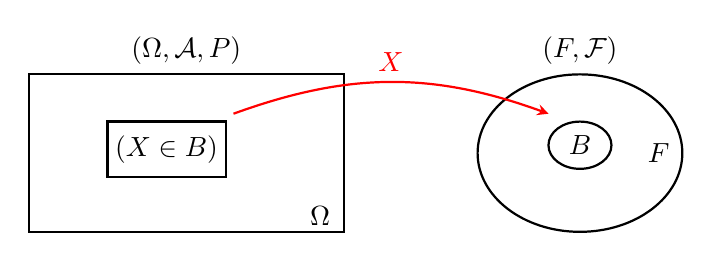
\begin{tikzpicture}[x=1cm,y=1cm,>=stealth,thick]

  % --- Spazio campionario (Omega) ---
  \draw[thick] (0,0) rectangle (4,2);
  \node at (3.7,0.2) {$\Omega$};
  \node at (2,2.3) {$(\Omega, \mathcal{A}, \mathbb{P})$};

  % --- Evento (X in B) all'interno di Omega ---
  \draw[thick] (1,0.7) rectangle (2.5,1.4);
  \node at (1.75,1.05) {$(X \in B)$};

  % --- Spazio dei valori (F) ---
  \draw[thick] (7,1) ellipse (1.3 and 1.0);
  \node at (7,2.3) {$(F, \mathcal{F})$};
  \node at (8,1) {$F$};

  % --- Sottoinsieme B ---
  \draw[thick] (7,1.1) ellipse (0.4 and 0.3);
  \node at (7,1.1) {$B$};

  % --- Freccia X ---
  \draw[red,->,thick,bend left=20] (2.6,1.5) to node[above,sloped,pos=0.5] {$X$} (6.6,1.5);

\end{tikzpicture}
\end{figure}

\noindent Sorge dunque la necessità di \emph{trasferire la misura di probabilità} dallo spazio degli esiti
allo spazio dei valori della variabile aleatoria,
in modo da poter calcolare probabilità del tipo
\[
\mathbb{P}(X \in B), \qquad B \in \mathcal{F}.
\]
Tale misura indotta, che traduce la distribuzione di probabilità di $\mathbb{P}$ attraverso $X$,
viene chiamata \emph{legge (o distribuzione) di $X$}.

\begin{definizione}
    Sia $X : (\Omega, \mathcal{A}, \mathbb{P}) \to (F, \mathcal{F})$ una variabile aleatoria. Si definisce \textit{legge di $X$} la funzione:
    \[P^X:\mathcal{F}\to [0, 1]\qquad \text{tale che}\qquad P^X(B) = \mathbb{P}(X\in B)\quad \forall B\in\mathcal{F}\]
\end{definizione}

\begin{proposizione}
    La legge di una variabile aleatoria \(\;P^X:\mathcal{F}\to [0, 1]\) è una probabilità
    \begin{dimostrazione}
    Ci basta dimostrare che $P^X(F) = 1$ e che valga la $\sigma$--additività.
    \begin{itemize}
        \item $P^X(F) \overset{\text{def}}{=} \mathbb{P}(X\in F) = \mathbb{P}(\Omega) = 1$
        \item Dato $(B_n)_{n\geq1}\subseteq\mathcal{F}\;$ tali che $\;B_h\cap B_k=\varnothing\;\forall h\neq k$, allora avremo che:
        \[P^X\left(\bigcup_{n=1}^\infty B_n\right) = \mathbb{P}\left(X\in\bigcup_{n=1}^\infty B_n\right) = \mathbb{P}\left(\bigcup_{n=1}^\infty(X\in B_n)\right)=\sum_{n=1}^\infty \mathbb{P}(X\in B_n)= \sum_{n=1}^\infty P^X(B_n)\]
    \end{itemize}
    \end{dimostrazione}
\end{proposizione}

Questa proposizione è fondamentale, in quanto se $X:(\Omega, \mathcal{A}, \mathbb{P})\to (F, \mathcal{F}) $ è una variabile aleatoria, allora possiamo vedere $(F, \mathcal{F}, P^X)$ come uno spazio di probabilità.\\
\\
Essendo $P^X$ una probabilità, possiamo quindi definire la funzione di ripartizione associata alla variabile aleatoria $X$:
\begin{definizione}
    Sia $X:(\Omega, \mathcal{A}, \mathbb{P})\to (\mathbb{R}, \mathcal{B}(\mathbb{R}))$ una variabile aleatoria reale, allora si definisce \textit{Funzione di Ripartizione di $X$} la funzione:
    \[F_X: \mathbb{R}\to [0, 1]\quad \text{data da}\quad F_X(t) = P^X((-\infty, t]) = \mathbb{P}(X\leq t)\]
\end{definizione}\bigskip

\begin{esempio}
Facciamo qualche esempio per capire meglio.\\
\(\bigstar\) Sia $X$ la somma dei risultati di due dadi, allora avremo che:
\[\Omega = \{1, ..., 6\}^2,\quad \mathcal{A} = 2^\Omega, \quad \mathbb{P} = \mathbb{P}_{\text{UNIF}};\qquad
\begin{array}{rcl}
X:\Omega & \to & \mathbb{R}\\[2pt]
(h,k) & \mapsto & h + k
\end{array}
, \quad \text{Im}(X)=\{2, ..., 12\}\]
Si vuole trovare $F_X$ e dire dire se $P^X$ è discreta o meno.
\begin{enumerate}
            \item Si ha chiaramente che $P^X(\{k\}) = \mathbb{P}(X\in \{k\}) = \mathbb{P}(X=k)$ con $k=2, ..., 12$.\\
            Quindi:
            \[P^X(\{k\}) = \mathbb{P}(\{(h, l)\in \Omega \mid h+l=k\}) = \begin{cases}
                \frac{k-1}{36}, \quad &\text{se } k \in [2, 6]\\
                \frac{13-k}{36}, \quad &\text{se } k \in [7, 12]
            \end{cases}\]

        Il perché di questo fatto risulta essere chiaro andando a costruire il reticolo dell somme ed il corrispondente istogramma delle frequenze.
\begin{figure}[H]
\centering
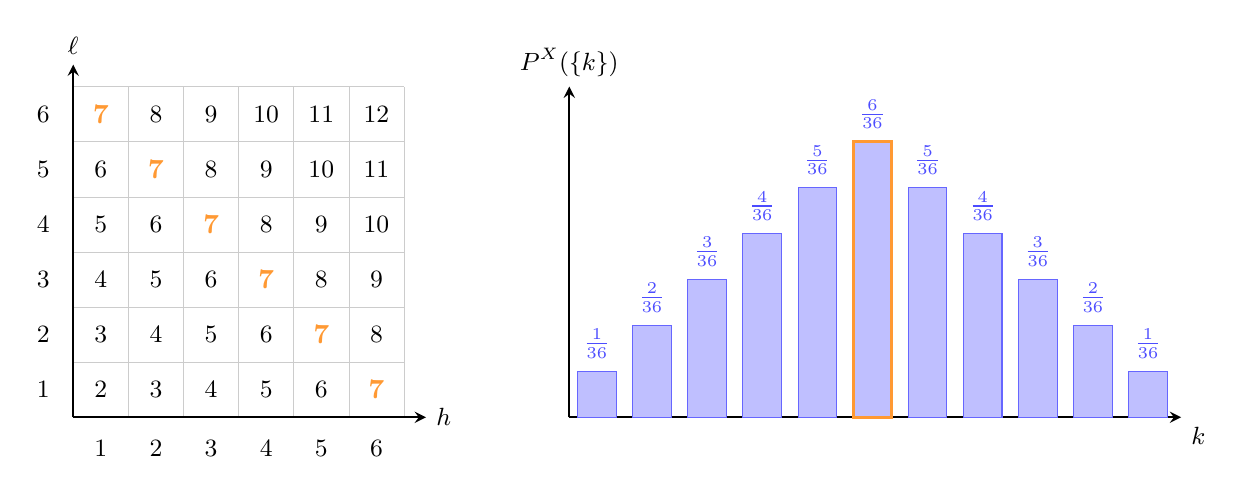
\begin{tikzpicture}[scale=0.7,>=stealth,font=\small]

% --- Parametro: somma da evidenziare (2..12)
\def\ksum{7}

% ================== Pannello A: reticolo ==================
\begin{scope}
  % Griglia e assi
  \draw[step=1cm, gray!40, very thin] (0,0) grid (6,6);
  \draw[->,thick] (0,0) -- (6.4,0) node[right] {$h$};
  \draw[->,thick] (0,0) -- (0,6.4) node[above] {$\ell$};

  % Tacche sugli assi
  \foreach \x in {1,...,6} \node[below] at (\x-0.5,-0.25) {\x};
  \foreach \y in {1,...,6} \node[left]  at (-0.25,\y-0.5) {\y};

  % Somme in ogni cella
  \foreach \h in {1,...,6}{
    \foreach \l in {1,...,6}{
      \pgfmathtruncatemacro{\somma}{\h+\l}
      \ifnum\somma=\ksum
        \node[orange!80, font=\bfseries] at (\h-0.5,\l-0.5) {\somma};
      \else
        \node at (\h-0.5,\l-0.5) {\somma};
      \fi
    }
  }

\end{scope}

% ================== Pannello B: istogramma P^X(k) ==================
% Scala indipendente per avere barre leggibili
\begin{scope}[xshift=7.5cm, x=1cm, y=5.0cm] 
  % Assi
  \draw[->,thick] (1.5,0) -- (12.6,0) node[below right] {$k$};
  \draw[->,thick] (1.5,0) -- (1.5,1.2) node[above] {$P^X(\{k\})$};

  % Barre k=2..12 con altezza c/6 (dove c = numero di coppie con somma k)
  \foreach \k in {2,...,12}{
    \pgfmathtruncatemacro{\c}{min(\k-1,13-\k)} % conteggi: 1,2,3,4,5,6,5,...
    \pgfmathsetmacro{\h}{\c/6}                  % normalizza: max = 1
    \draw[fill=blue!25,draw=blue!60] (\k-0.35,0) rectangle (\k+0.35,\h);
    \node[blue!70] at (\k,\h+0.1) {$\frac{\c}{36}$};
  }

  % Coordinata della barra corrispondente a ksum (per la freccia)
  \pgfmathtruncatemacro{\ck}{min(\ksum-1,13-\ksum)}
  \pgfmathsetmacro{\hk}{\ck/6}
  \coordinate (BarTop) at (\ksum,\hk);

  % Evidenzia la barra selezionata
  \draw[orange!80,very thick] (\ksum-0.35,0) rectangle (\ksum+0.35,\hk);  
\end{scope}


\end{tikzpicture}
\end{figure}


Si vede che per i risultati di $X$ fino a $7$, la frequenza (e quindi la probabilità) aumenta sempre di più; il contrario vale per i valori delle somme tra $7$ e $12$, la quale frequenza diminuisce.\\
La funzione di ripartizione di $X$ risulta essere quindi:
\[F_X(t) = \mathbb{P}(X\leq t) = 
\begin{cases}
    \sum_{k=2}^{\lfloor t\rfloor} P^X(\{k\}), \quad &\text{se } t\geq2\\
    0 &\text{se } t<2
\end{cases}\]

\item Inoltre $P^X$ risulta essere una probabilità discreta in quanto $F_X$ rispetta tutte le condizioni della Proposizione \ref{prop:fdr}.
\end{enumerate}

\(\bigstar\) Siano $\Omega = F = \mathbb{R}, \; \mathcal{A}= \mathcal{F} = \mathcal{B}(\mathbb{R})$. Si consideri $\mathbb{P} \sim \mathcal{E}(\lambda)$, ossia che: \(\;F(t) = (1-e^{-\lambda t}) \mathbb{I}_{[0, +\infty]}(t)\).\\
Sia inoltre $X:\mathbb{R}\to\mathbb{R}\;$ tale che $\;X(w) = \lfloor w\rfloor + 1$.\\
\\
Si vuole trovare $P^X$, e chiarire se sia discreta o meno.\\
\\
Come abbiamo già visto, $\text{Im}(X) = \mathbb{Z}$; si osservi inoltre che $\mathbb{P}((-\infty, 0])$ = F(0) = 0.\\
    Avremo quindi che $\forall k \geq 1$:
    \begin{align*}
        P^X (\{k\})&= \mathbb{P}(X=k) = \mathbb{P}(w\in\mathbb{R}\mid \lfloor w \rfloor = k-1) = \mathbb{P}([k-1, k)) \\
        & = F(k^-) - F((k-1)^-) \overset{\text{continuità}}{=} F(k) - F(k-1) \\
        & = (e^{-\lambda})^{k-1}(1-e^{-\lambda})
    \end{align*}
La quale è una \textit{legge Geometrica} di parametro $(1-e^{-\lambda}):\; X\sim G(1-e^{-\lambda})$, che per definizione è rappresenta una probabilità discreta.
\end{esempio}

\section{Relazioni fra Variabili Aleatorie: Uguaglianza Quasi Certa ed in Legge}
Nel calcolo delle probabilità, quando si opera con variabili aleatorie, non sempre è necessario che due funzioni coincidano esattamente in ogni punto dello spazio campionario per essere considerate “uguali” dal punto di vista probabilistico.
Ciò che conta, infatti, non è il comportamento puntuale della funzione in ogni singolo esito $w\in\Omega$, ma il comportamento su insiemi che hanno probabilità positiva.

\medskip
\noindent Per questo motivo si introduce il concetto di uguaglianza quasi certa (o uguaglianza $\mathbb{P}$--quasi ovunque), che consente di considerare trascurabili (dal punto di vista probabilistico) le differenze che si verificano su un insieme di probabilità nulla.\\
\\
\noindent Questa nozione (come avremo modo di approfondire più avanti) è fondamentale perché, nella teoria della misura e dell’integrazione, le funzioni che differiscono solo su insiemi di misura nulla vengono considerate equivalenti: la probabilità è essa stessa una misura, e quindi eredita questa stessa logica.

\medskip
\noindent L’uguaglianza quasi certa permette dunque di trattare come “identiche” due variabili che, pur non coincidendo puntualmente, hanno lo stesso comportamento probabilistico e generano gli stessi risultati integrali.\\
\\
Introdurremo anche un altro tipo di uguaglianza, ovvero quella in Legge, che ci permetterà di considerare variabili aleatorie che hanno domini differenti.\\

\begin{esempio}
    Se prendiamo due funzioni uguali ovunque, tranne che in un punto, queste risulteranno essere uguali quasi certamente, in quanto la misura (probabilità) di un punto è zero.
    \begin{figure}[H]
\centering
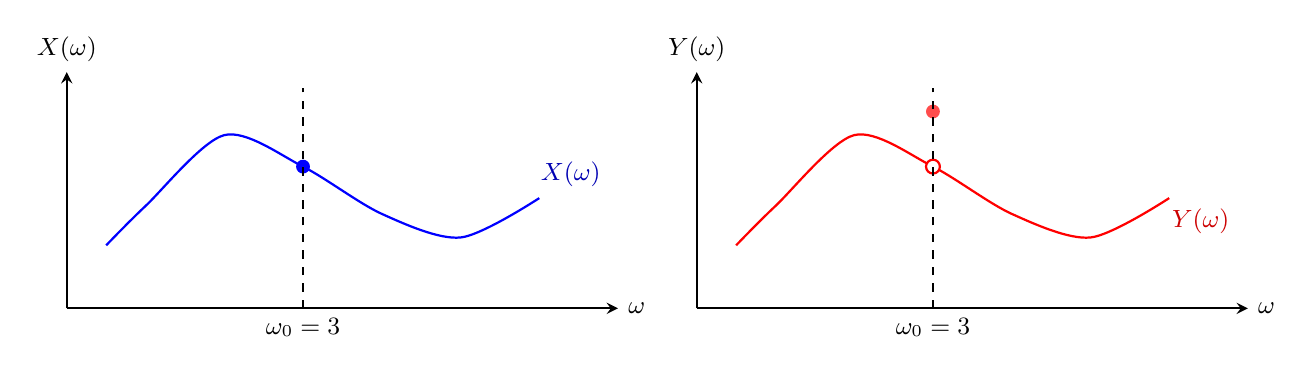
\begin{tikzpicture}[x=1cm,y=1cm,font=\small,>=stealth]

% ==================== Grafico 1: X(ω) ====================
\begin{scope}
  % Assi
  \draw[->,thick] (0,0) -- (7,0) node[right] {$\omega$};
  \draw[->,thick] (0,0) -- (0,3) node[above] {$X(\omega)$};

  % Funzione X(ω)
  \draw[blue,thick,smooth]
    plot coordinates {(0.5,0.8) (1.0,1.3) (2.0,2.2) (3.0,1.8)
                      (4.0,1.2) (5.0,0.9) (6.0,1.4)};
  \fill[blue] (3,1.8) circle (2.5pt);
  \node[blue!70!black] at (6.4,1.7) {$X(\omega)$};

  % Linea verticale e etichetta ω0=3
  \draw[dashed,thick] (3,0) -- (3,2.8);
  \node[below] at (3,0) {$\omega_0=3$};
\end{scope}


% ==================== Grafico 2: Y(ω) ====================
\begin{scope}[xshift=8cm]
  % Assi
  \draw[->,thick] (0,0) -- (7,0) node[right] {$\omega$};
  \draw[->,thick] (0,0) -- (0,3) node[above] {$Y(\omega)$};

  % Funzione Y(ω) (uguale a X tranne in ω0=3)
  \draw[red,thick,smooth]
    plot coordinates {(0.5,0.8) (1.0,1.3) (2.0,2.2) (3.0,1.8)
                      (4.0,1.2) (5.0,0.9) (6.0,1.4)};
  \fill[red!70] (3,2.5) circle (2.5pt);
  \filldraw[white, draw=red, thick] (3,1.8) circle (2.5pt);
  \node[red!80!black] at (6.4,1.1) {$Y(\omega)$};

  % Linea verticale e etichetta ω0=3
  \draw[dashed,thick] (3,0) -- (3,2.8);
  \node[below] at (3,0) {$\omega_0=3$};
\end{scope}

\end{tikzpicture}
\caption{Esempio di due funzioni uguali quasi certamente}
\end{figure}
\end{esempio}

\bigskip
\noindent Cerchiamo ora di dare delle definizioni formali a questi concetti.
\begin{definizione}
\label{def:eq}
    Siano $X, Y:(\Omega, \mathcal{A}, \mathbb{P})\to(\mathbb{R}, \mathcal{B}(\mathbb{R}))$ due variabili aleatorie. $X$ ed $Y$ sono uguali se:
    \[X(w) = Y(w)\qquad \forall w\in\Omega\]
\end{definizione}

\begin{definizione}[Uguaglianza in Legge]
\label{def:eqlegge}
    Siano $X:(\Omega_1, \mathcal{A}_1, \mathbb{P}_1)\to (F, \mathcal{F})\;\;$ e $\;\;Y:(\Omega_2, \mathcal{A}_2, \mathbb{P}_2)\to (F, \mathcal{F})$ due variabili aleatorie. Si dice che hanno la stessa legge se:
    \[P^X=P^Y\]
    Ossia che: $\quad \forall B\in\mathcal{F}\quad P^X(B)=P^Y(B)$
\end{definizione}

Si presti attenzione al fatto che nella Definizione \ref{def:eqlegge}, $X$ e $Y$ \textbf{possono partire da spazi differenti}, \textbf{ma comunque devono arrivare nello stesso spazio misurabile}; per quanto riguarda la Definizione \ref{def:eq}, se le variabili aleatorie partissero da spazi differenti, la definizione perderebbe di senso.

\medskip
\noindent Questo può essere interpretato come un primo campanello d'allarme sul fatto che l'uguaglianza ``classica'' sia troppo stringente, e quindi necessitiamo di un altri tipi di uguaglianze meno vincolanti.
\begin{definizione}[Uguaglianza quasi certa]
Siano $X:\Omega\to F$, e $Y:\Omega \to F$ due variabili aleatorie. Si dice che $X$ ed $Y$ sono quasi certamente uguali se:
\[\exists \;A\in\mathcal{A} \;\text{ con }\;\mathbb{P}(A) = 1\qquad \text{tale che: }\qquad X(w) = Y(w)\quad \forall w\in A\]
\\
O alternativamente, solo nel caso in cui  $F=\mathbb{R}, \mathbb{R}^n, \;$ $X$ ed $Y$ sono uguali q.c. se:\(\qquad \mathbb{P}(X=Y) = 1\)
\end{definizione}

Si noti che l'uguaglianza quasi certa è legata alla probabilità sulla quale le due variabili aleatorie sono definite; se cambio lo spazio di probabilità, potrebbe essere che $X$ e $Y$ non siano più q.c. uguali.

\medskip
\noindent Anche in questo caso, affinché la definizione abbia senso matematico, è necessario che le due variabili aleatorie abbiano lo stesso dominio.\\
\\
Da un punto di vista modellistico, $X$ e $Y$ \textbf{risultano indistinguibili alla probabilità} $\mathbb{P}$.

\begin{esempio}
    Siano $\Omega = F = \mathbb{R}, \; \mathcal{A}= \mathcal{F} = \mathcal{B}(\mathbb{R})$. Si consideri $\mathbb{P} \sim \mathcal{E}(\lambda)$, e si prendano le tre V.A. definite come segue:
    \[\left.
    \begin{aligned}
        X_1(w) &= w \\
        X_2(w) &= |w|\\
        X_3(w) &= w\cdot\mathbb{I}_{\mathbb{R}\setminus\mathbb{Q}}
    \end{aligned}
    \qquad \right\} \qquad \Rightarrow \quad X_1\neq X_2\neq X_3
    \]
    Tuttavia $X_1 \overset{q.c.}{=}X_2\overset{q.c.}{=}X_3,\;$ difatti si ha che:
    \[(X_1 = X_3) = (\mathbb{R}\setminus\mathbb{Q})\]
    \[\Rightarrow\quad \mathbb{P}(X_1 = X_3) = \mathbb{P}(\mathbb{R}\setminus\mathbb{Q}) = \mathbb{P}(\mathbb{R}) - \mathbb{P}(\mathbb{Q}) = 1-0=1 \quad \Rightarrow\quad X_1 \overset{q.c.}{=}X_3\]
    dato che $\mathbb{P}(\mathbb{Q}) = \mathbb{P}(\bigcup_{n=1}^\infty\{q_n\}) = \sum_{n=1}^\infty \mathbb{P}(\{q_n\}) = 0$.\\
    \\
    Allo stesso modo si dimostra che $X_1 \overset{q.c.}{=}X_2$ e di conseguenza $X_2 \overset{q.c.}{=}X_3$
\end{esempio}

\newpage
\noindent Possiamo chiederci arrivati a questo punto: \textit{quale è la relazione tra i tipi di uguaglianze che abbiamo visto?}

\begin{proposizione}
    $X=Y\quad\Rightarrow\quad X\overset{q.c.}{=}Y \quad\Rightarrow\quad P^X=P^Y $
    \begin{dimostrazione}
        La prima implicazione è triviale, pertanto lasciata al lettore. LOL\\
        Per quanto riguarda la seconda, $\;\forall B\in \mathcal{F}$:
        \begin{align*}
            P^X(B) &= \mathbb{P}(X\in B) = \mathbb{P}(X\in B\;\; \cap\;\; X=Y) + \cancelto{0}{\mathbb{P}(X\in B\;\; \cap\;\; X\neq Y)}\\
            & = \mathbb{P}(X\in B\;\; \cap\;\; X=Y) = \mathbb{P}(Y\in B\;\; \cap\;\; X=Y) = \mathbb{P}(Y\in B)\\
            & = P^Y(B)
        \end{align*}
    \end{dimostrazione}
\end{proposizione}

\bigskip
\noindent Si faccia attenzione ad alcune osservazioni.\\
\\
\(\bigstar\) Per conoscere $P^X$ è sufficiente conoscere $X(w)\;\forall w\in A$, dove $\mathbb{P}(A)=1$.\\
Quindi se avessimo una variabile aleatoria $Y$ definita come
\[Y(w) = \begin{cases}
    X(w), \quad &\text{se } w\in A, \;\text{con }\;\mathbb{P}(A)=1\\
    0 &\text{se }w \notin A
\end{cases}\]
potremmo senz'altro concludere che $Y\overset{q.c.}{=}X$.\\
\\
\(\bigstar\) In generale possiamo dire che una qualunque proprietà che dipende da $w\in\Omega$ vale ``quasi certamente'' se: 
\[\exists A\in\mathcal{A}, \;\mathbb{P}(A)=1\qquad\text{tale che la proprietà valga }\forall w \in A\]
\begin{esempio}
    Si consideri:
    \[\Omega=F=\mathbb{R};\qquad \mathcal{A}=\mathcal{F} = \mathcal{B};\qquad \mathbb{P}\sim \mathcal{U}([0, 1])\;\Rightarrow\;F(t) = t\cdot \mathbb{I}_{[0, 1]} + \mathbb{I}_{(1, +\infty)}\]


    Consideriamo ora $X(w)=w, \; \forall w\in \Omega = \mathbb{R}$. Si ha che $\text{Im}(X) = \mathbb{R}$, tuttavia:
    \[\mathbb{P}(X\in [0, 1]) = \mathbb{P}(w\in\mathbb{R}\mid X(w) = w\in[0, 1]) = \mathbb{P}([0, 1]) = F(1) - F(0) = 1\]
    $\Rightarrow\quad$Possiamo affermare che $X\in[0, 1]$ sia una proprietà che vale quasi certamente
\end{esempio}



